\documentclass{beamer}
\usetheme{Madrid}
\usepackage[spanish]{babel}
\usepackage{amsmath}
\usepackage{caption}
\usepackage{ragged2e}  
\usepackage{multicol}
\setbeamertemplate{caption}[numbered]




% Paquete para posicionar el logo
\usepackage[absolute,overlay]{textpos} 

% Paquete para importar imágenes
\usepackage{graphicx}  

\setbeamertemplate{frametitle}{
  \begin{beamercolorbox}[sep=0.3cm,center,wd=\paperwidth]{frametitle}
    \usebeamerfont{frametitle}\parbox[c][0.8cm][c]{.8\textwidth}{\insertframetitle}\hfill
    \raisebox{-0.3\height}{
\includegraphics[height=0.8cm]{Logos/MarcaBlanco.png}}
  \end{beamercolorbox}
}


\def\supervisor{Dr. Carlos Fuhrhop}
\def\course{Control Avanzado}

\title{¿Se puede controlar la epidemia de COVID-19 basándose en los informes de pruebas diarios?}
\author{Ing. Rodrigo Salazar,M Elvin Soto}
\institute{UACH}
\date{\today}

% Modificación de la planilla del titulo
\setbeamertemplate{title page}{
  \vbox{}
  \vfill
  \begin{centering}
    %Para llamar a los diferentes logotipos del titulo
    
\includegraphics[height=1.1cm]{Logos/electronica-color.png} \hspace{0.8cm}  
    
\includegraphics[height=1.5cm]{Logos/UACh_Marcacolor.png} \hspace{0.5cm} 
    
\includegraphics[height=0.9cm]{Logos/MarcaColor.png}  
    \par
    \vskip1.5em%
    {\usebeamercolor[fg]{titlegraphic}\inserttitlegraphic\par}
    \begin{beamercolorbox}[sep=8pt,center,colsep=-4bp,rounded=true,shadow=true]{title}
      \usebeamerfont{title}\inserttitle\par%
      \ifx\insertsubtitle\@empty%
      \else%
        \vskip0.25em%
        {\usebeamerfont{subtitle}\usebeamercolor[fg]{subtitle}\insertsubtitle\par}%
      \fi%     
    \end{beamercolorbox}%
    \vskip1em\par
    \begin{beamercolorbox}[sep=8pt,center,colsep=-4bp,rounded=true,shadow=true]{author}
      \usebeamerfont{author}\insertauthor
    \end{beamercolorbox}
    \begin{beamercolorbox}[sep=8pt,center,colsep=-4bp,rounded=true,shadow=true]{author}
      \usebeamerfont{author}Profesor: \supervisor
    \end{beamercolorbox}
    \begin{beamercolorbox}[sep=8pt,center,colsep=-4bp,rounded=true,shadow=true]{author}
        \usebeamerfont{author}Curso: \course
    \end{beamercolorbox}
    \begin{beamercolorbox}[sep=8pt,center,colsep=-4bp,rounded=true,shadow=true]{institute}
      \usebeamerfont{institute}\insertinstitute
    \end{beamercolorbox}
    \begin{beamercolorbox}[sep=8pt,center,colsep=-4bp,rounded=true,shadow=true]{date}
      \usebeamerfont{date}\insertdate
    \end{beamercolorbox}\vskip0.5em
    {\usebeamercolor[fg]{titlegraphic}\inserttitlegraphic\par}
    \par
    \vfill
  \end{centering}
}

\begin{document}
\begin{frame}
  \titlepage
\end{frame}


\begin{frame}
  \frametitle{Contenido}
  \tableofcontents
\end{frame}


\section{Introducción: Vista Previa}
\begin{frame}{Introducción}

% El \begin{justify} para dejar el texto en Justificado.
\begin{justify}  
El primer brote de la epidemia del virus COVID-19 tuvo lugar en China, comenzando a finales de 2019, en donde causó una pandemia global con efectos disruptivos en la salud pública, la vida social y la economía.

\vspace{0.3cm}
Se han propuesto una amplia variedad de modelos matemáticos para describir la evolución dinámica de las epidemias, incluyendo una algunos bastante sofisticados.

\vspace{0.3cm}
El análisis de estos modelos permite predecir la evolución de la enfermedad con el tiempo y lo más importante, cómo depende de los parámetros del modelo.

\end{justify}
\end{frame}


\begin{frame}{Introducción}

% El \begin{justify} para dejar el texto en Justificado.
\begin{justify}  
Los modelos epidemiológicos se utilizan ampliamente para diseñar estrategias de vacunación y tratamiento basadas en el control óptimo. 

\vspace{0.3cm}
También se pueden utilizar para diseñar estrategias de vacunación con retroalimentación, o incluso estrategias de retroalimentación que combinan diferentes acciones como vacunación, tratamiento y sacrificio. 

\vspace{0.3cm}
Algunos estudios tienen en cuenta los efectos de los cambios de comportamiento en la evolución de una epidemia. 

\vspace{0.3cm}
La mayoría de los modelos utilizados para estudiar estrategias de control están formulados en términos de ecuaciones diferenciales ordinarias, por ejemplo, los modelos SIR y SEIR clásicos y sus variantes. 


\end{justify}
\end{frame}


\begin{frame}{Introducción}
\begin{justify}

El objetivo de este artículo es evaluar la controlabilidad del brote de COVID-19, asumiendo que la población está adecuadamente mezclada (homogenización) y que las decisiones de las medidas de salud pública por parte de las autoridades se basan en informes diarios de pruebas de hisopado positivas, casos activos y casos totales. 

\vspace{0.3cm}
Con este fin, se presenta un modelo simplificado, que busca capturar la dinámica fundamental del proceso que es relevante para el control de retroalimentación, y resulta estar fuertemente afectado por el retraso temporal.

\end{justify}
\end{frame}

\section{Derivación del modelo}
\begin{frame}{Derivación del modelo}
\begin{justify}
{\footnotesize

Los modelos de la epidemia de COVID-19, se basan en principios fundamentales, sus ecuaciones describen la evolución temporal de diferentes categorías de sujetos, basándose en los mecanismos conocidos de infección, recuperación y cuidado de los pacientes. 

\vspace{0.2 cm}
Las políticas públicas basadas en tales modelos deben ser adaptadas y corregidas en función del resultado observado. Los indicadores utilizados por los tomadores de decisiones públicas incluyen informes diarios de: 

\begin{itemize}
 
 \vspace{0.3 cm}
    \item\textbf{Nuevas pruebas de hisopo positivas.} 

 \vspace{0.1 cm}
    \item\textbf{Número actual de sujetos infectados,} 

 \vspace{0.1 cm}
    \item\textbf{Número total de casos informados.} 

\end{itemize}

\vspace{0.3cm}
La pregunta crucial entonces es: 

\vspace{0.3cm}
¿Es factible el control de retroalimentación en tal sistema?


}

\end{justify}
\end{frame}

% \Huge, \huge, \LARGE, \Large, \large, \normalsize, \small, \footnotesize, \scriptsize, \tiny

\begin{frame}{Derivación del modelo}
\begin{justify}
{\footnotesize

Para responder a esta pregunta, aquí se deriva un modelo simplificado para capturar la dinámica fundamental de la epidemia relevante para el diseño de la política de retroalimentación, en particular la relación dinámica entre las NPIs (Intervención no farmacéutica) y la respuesta de los tres indicadores mencionados anteriormente.

\vspace{0.2 cm}
El punto de partida es el modelo SEIR básico con la adición de un compartimento adicional L:
 
\begin{equation}
    \frac{dS}{dt} = -\frac{\beta IS}{N}
\end{equation}

\begin{equation}
    \frac{dE}{dt} = \frac{\beta IS}{N} - \epsilon E
\end{equation}

\begin{equation}
    \frac{dI}{dt} = \epsilon E - \gamma I
\end{equation}

\begin{equation}
    \frac{dL}{dt} = \gamma I - \delta L
\end{equation}

\begin{equation}
    \frac{dR}{dt} = \delta L
\end{equation}
}


\end{justify}
\end{frame}


\begin{frame}{Derivación del modelo}
\begin{justify}
\small
Donde:
{\footnotesize
\begin{itemize}
    \item $N$: La población total.
    \item $S$: El número de individuos Susceptibles.
    \item $E$: El número de individuos Expuestos que han contraído la infección pero aún no son infecciosos.
    \item $I$: El número de individuos Infectados.
    \item $L$: El número de sujetos que aún están infectados pero ya no son infecciosos debido a hospitalización, cuarentena, o porque los sujetos infectados son mayormente infecciosos solo durante los primeros días después del final del período de latencia.
    \item $R$: El número de individuos Recuperados y resistentes a futuras infecciones.
    \item $\beta$: La tasa de transmisión efectiva.
    \item $\epsilon$: La tasa inversa del período promedio de incubación antes de que uno se vuelva infeccioso.
    \item $\gamma$: La tasa inversa del tiempo promedio que los sujetos infectados pasan siendo infecciosos.
    \item $\delta$: La tasa inversa del tiempo promedio que los sujetos infectados permanecen enfermos pero no infecciosos.
\end{itemize}

}
\end{justify}
\end{frame}


\begin{frame}{Derivación del modelo}
\begin{justify}
Donde:
\begin{itemize}
    \item Si se hace S(t)/N $\approx$ 1 y se deshace de una ecuación y la variable S.
    \item De hecho, una parte importante de la población puede no ser susceptible a priori, por ejemplo, por motivos genéticos. Sin embargo, a falta de evidencia concreta de este hecho, el principio de precaución sugiere considerar el peor caso S(t)/N = 1.
    \item  $\beta(u(t), d(t))$ una función.
    \item u(t) indica la intensidad de las políticas públicas respecto a las restricciones.
    \item d(t) es una perturbación del sistema.
\end{itemize}
\end{justify}
\end{frame}


\begin{frame}{Derivación del modelo}
\begin{justify}
\vspace{0.3cm}
\item El sistema quedaría:
\begin{align}
    \frac{dE}{dt} &= \beta(u(t), d(t))I - \epsilon E, \label{eq:Et} \\[10pt]
    \frac{dI}{dt} &= \epsilon E - \gamma I, \label{eq:It} \\[10pt]
    \frac{dL}{dt} &= \gamma I - \delta L, \label{eq:Lt} \\[10pt]
    \frac{dR}{dt} &= \delta L, \label{eq:Tt} \\[10pt]
\end{align}
\begin{table}[htbp]
  \centering
  \caption{Tabla de Ejemplo}
  \begin{tabular}{|c|l|r|}
    \hline
    \textbf{Encabezado 1} & \textbf{Encabezado 2} & \textbf{Encabezado 3} \\
    \hline
    1 & Contenido & \$100 \\
    2 & Otra fila & \$200 \\
    3 & Más datos & \$300 \\
    \hline
  \end{tabular}
\end{table}

\end{justify}
\end{frame}

\begin{frame}{Derivación del modelo}
\begin{justify}
\vspace{0.3cm}
\item Los parámetros del modelo queda:
\begin{table}
    \centering
    \caption{Datos de parámetros del modelo epidemilógico estudiado}
    \begin{tabular}{|c|c|c|c|c|c|}
        \hline
        \textbf{Pais} & \textbf{Periodo} & \textbf{$\beta_o$} &
        \textbf{$1/\lambda$} &
        \textbf{$1/\epsilon$} &
        \textbf{$1/\delta$}  \\
        \hline
        China & 18/01/20-11/02/20 & 1.6 & 2.5 & 5.0 & N/A \\
        \hline
        Italia & 22/02/20-01/05/20 & 1.3 & 3.1 & 4.3 & 33 \\
        \hline
        Francia & 28/02/20-03/05/20 & 1.3 & 2.9 & 5.0 & 29 \\
        \hline
        UK & 01/02/20-10/05/20 & 1.28 & 2.8 & 6.2 & N/A \\
        \hline
    \end{tabular}
\end{table}
\end{justify}
\end{frame}

\begin{frame}{Derivación del modelo}
\begin{justify}
\begin{figure}
    \centering
    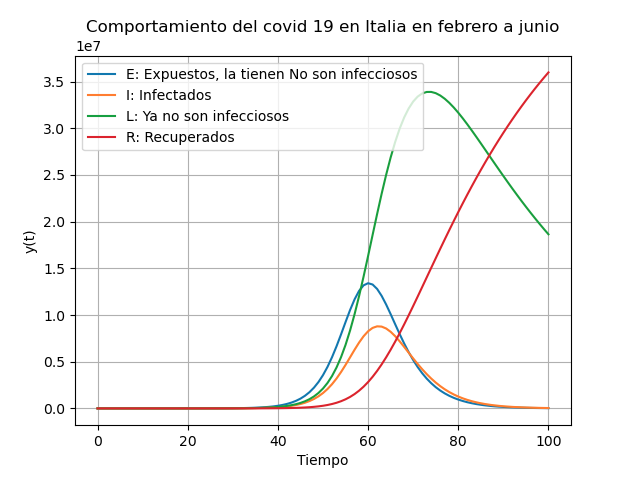
\includegraphics[width=0.7\textwidth]{ModeloItaliaCOVID.png}
    \caption{Modelo COVID-19- Caso Italia. Resuelto con RK-4}
    \label{fig:CovidItalia}
\end{figure}
\end{justify}
\end{frame}


\begin{frame}{Derivación del modelo}
\begin{justify}
{\footnotesize
Consideraciones:

\vspace{0.2cm}
\item Donde se llevó a cabo una prueba masiva, se encontró que aproximadamente el 40 \% de los sujetos que dieron positivo son completamente asintomáticos, a pesar de ser infecciosos.

\vspace{0.2cm}
\item las pruebas con hisopos tienen más del 20 \% de falsos negativos y algunos sujetos con síntomas leves pueden terminar no siendo testeados.

\vspace{0.2cm}
Podemos suponer que el parámetro variable en el tiempo $\beta$ es en realidad una función de una variable representativa manipulada $u(t)$, donde esta última indica la intensidad de las medidas de salud pública adoptadas en una escala de 0 al 1.

\vspace{0.2cm}
La función $\beta(.)$ disminuye monotónicamente desde el valor $\beta_0$, cuando no se aplican restricciones sociales, hasta cero, correspondiente al aislamiento total de cada persona en el país.

\vspace{0.2cm}
Hay una considerable incertidumbre involucrada en la estimación de los efectos de diferentes intervenciones en términos de reducción de $\beta$ o equivalentemente de $R_t$.


}
\end{justify}
\end{frame}



\begin{frame}{Derivación del modelo}
\begin{justify}
\small
 El modelo orientado al control puede formularse como un sistema en espacio-estado y salidas con retardo

 \vspace{0.2cm}
{\footnotesize
\begin{align}
    \frac{dE_t}{dt} &= \beta(u(t), d(t))I_t - \epsilon E_t, & N_r(t) &= \epsilon E_t(t - \tau_m), \\[10pt]
    \frac{dI_t}{dt} &= \epsilon E_t - \gamma I_t, & A_r(t) &= I_t(t - \tau_m) + L_t(t - \tau_m), \\[10pt]
    \frac{dL_t}{dt} &= \gamma I_t - \delta L_t, & T_r(t) &= T_t(t - \tau_m), \\[10pt]
    \frac{dT_t}{dt} &= \epsilon E_t,
\end{align}

 \vspace{0.2cm}
Donde $\tau_m$ es el retraso total de medición, 
$N_r$ es el número de nuevos casos reportados diariamente, $A_r$ es el número de casos activos reportados y $T_r$ es el número total acumulado de informes de pruebas positivas.
}
\end{justify}
\end{frame}


\begin{frame}{Derivación del modelo}
\begin{justify}
{\footnotesize
Donde:
\begin{itemize}
\justifying
    \item $\beta(u, d)$ es una función.
    \vspace{0.3cm}
    \item $\epsilon$, $\gamma$ y $\delta$ son parámetros constantes.
    \vspace{0.3cm}
    \item $\tau_m=\tau_t+\tau_r$ es el retraso total de medición. Donde $\tau_t$ son los dias en que alguien se vuelve infeccioso y $\tau_r$ es el retraso en entregar un resultado de test.
    \vspace{0.3cm}
    \item La variable medida del proceso es el número de $N_r(t)$ de nuevos casos reportados diariamente afectado por $\tau_m$.
    \vspace{0.3cm}
    \item $A_r(t)$ de casos activos reportados, es decir, el número de sujetos para los cuales se ha recibido un informe de prueba positiva y aún no se ha emitido una prueba negativa.
    \vspace{0.3cm}
    \item $T_t(t)$ es el número total acumulado de informes de pruebas positivas. 
\end{itemize}
}

\end{justify}
\end{frame}



\begin{frame}{Validación y Ajuste}
\begin{justify}

{\footnotesize
Consideraciones:
\begin{itemize}
\justifying
    \item El objetivo del modelo es describir la respuesta dinámica de los indicadores de $N_r(t)$, $A_r(t)$ y $T_r(t)$ a la aplicación de NPIs por autoridades centrales y descritas por cambios de $u(t)$.
    \vspace{0.3cm}
    \item Se seleccionaron cuatro casos de brotes, todos caracterizados por cambios escalonados de $u(t)$ a nivel del gobierno central, con el fin de facilitar la validación, con datos tomados de China, Italia, Francia y el Reino Unido, que informa datos de autoridades nacionales.
    \vspace{0.3cm}
    \item En el caso de Italia y el Reino Unido, se introdujeron primero algunas restricciones parciales, lo que provocó una notable reducción retrasada del ritmo de aumento exponencial de nuevos casos.
    \vspace{0.3cm}
    \item Se asumió que $\beta = \beta_0$ en $t=0$, luego $\beta$ sufre una reducción escalonada a $\beta = \rho_1 \beta_0$ en $t= t_1$ y otra reducción adicional de  $\beta = \rho_2 \beta_0$ en $t_2$. Donde $\rho_1$ y $\rho_2$ son valores constantes correspondiente a los cambios en el escalón de control por políticas de restricción.
    \vspace{0.3cm}
    
\end{itemize}
}

\end{justify}
\end{frame}


\begin{frame}{Validación y Ajuste}
\begin{justify}

{\footnotesize
Consideraciones:
\begin{itemize}
\justifying
    \item Los parámetros del modelo se ajustaron manualmente para obtener un buen ajuste con los datos disponibles.
    \vspace{0.3cm}
    \item En particular, \( t_m \) se ajusta fácilmente para coincidir con el retraso entre el confinamiento y el pico de \( N_r(t) \).
    \vspace{0.3cm}
    \item \( R_t = \beta/\gamma \) y \( \rho_1 \) determinan las tasas de crecimiento en el comportamiento pre-confinamiento de \( N_r(t) \).
    \vspace{0.3cm}
    \item \( \rho_2 \) %, \( \gamma \) y \( \epsilon \)%
    determina la forma y la tasa de decaimiento del comportamiento post-confinamiento de \( N_r(t) \).
    \vspace{0.3cm}
    \item \( T_r(t) \) es la integral de \( N_r(t) \), y su ajuste ayuda a refinar el ajuste de los parámetros considerando la naturaleza ruidosa de \( N_r(t) \), que también se ve afectada por una oscilación semanal debido a la repetición de los horarios de laboratorio.
    \vspace{0.3cm}
    
\end{itemize}
}

\end{justify}
\end{frame}

\begin{frame}{Validación y Ajuste}
\begin{justify}
\small
{\footnotesize

\begin{figure}[H]
\centering
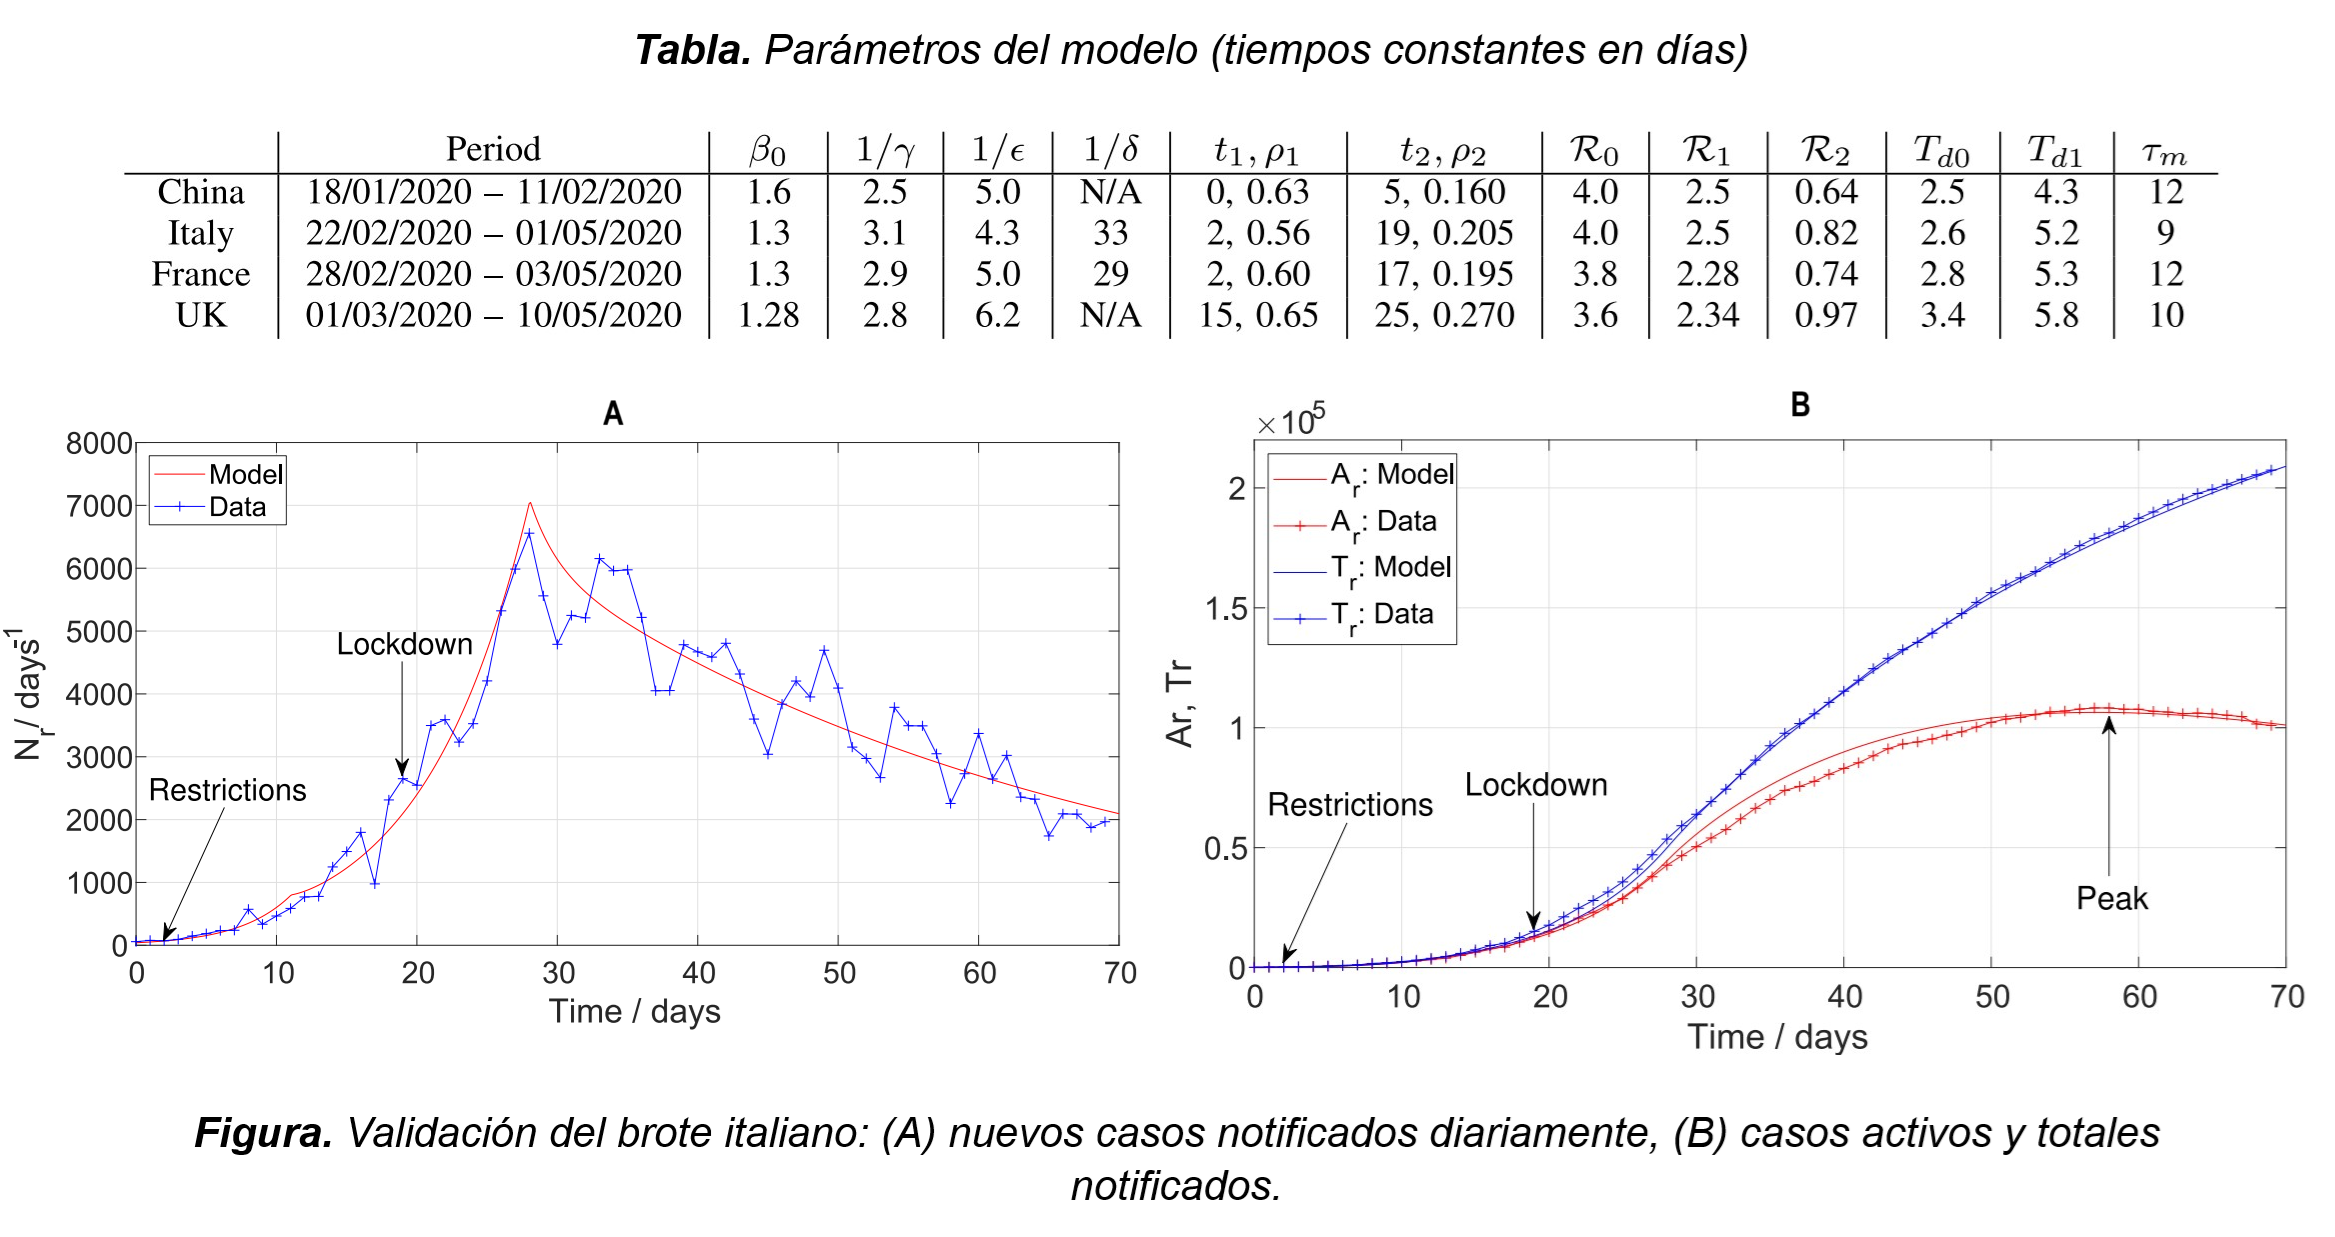
\includegraphics[width=0.95\textwidth]{imagen-simulacion.png}
\captionsetup{justification=centering}
\label{C2}
\end{figure}
}


\end{justify}
\end{frame}


\begin{frame}{Control: Estrategia de Supresión}
\begin{justify}
\small
Los efectos de la aplicación de las dos políticas de control delineadas en la Introducción serán ahora analizados. Las estrategias de control retroactivo no deben aplicarse sin consideración en sistemas inestables críticos para la seguridad.

\vspace{0.3cm}
La estrategia de supresión puede resumirse en los siguientes términos: tan pronto como \( A_r(t) \) alcance un valor \( A_s \), que es lo suficientemente alarmante para los tomadores de decisiones, se toman medidas drásticas de contención.
\[
u(t) =
\begin{cases}
0, & A_r(t) < A_s \\
\bar{u}, & A_r(t) \geq A_s
\end{cases}
\]

\vspace{0.3cm}
%Si el umbral \( A_s \) se cruza y \( \bar{u} \) es grande, entonces \( \beta(\bar{u})/\gamma < 1 \) implicando \( r < 0 \). Esto conduce a un sistema LTI homogéneo con autovalores negativos, lo que indica una disminución en el número de casos.%
\end{justify}
\end{frame}


\begin{frame}{Control: Estrategia de Supresión}
\begin{justify}
\small
El número de casos activos reportados \( A_r(t) \) y, por lo tanto, el número requerido de camas en hospitales y unidades de cuidados intensivos, dejará de aumentar exponencialmente después de \( t_m \) días, pero seguirá creciendo y alcanzará su pico más tarde debido a la constante de tiempo más lenta \( 1/\delta \).

\vspace{0.3cm}
Asumiendo que una fracción de casos activos requiere cuidados intensivos y que hay un número limitado de camas de cuidados intensivos disponibles, es crucial escoger un \( A_s \) adecuado. %Los políticos sin formación en modelado matemático pueden no comprender la importancia de actuar rápidamente.
%
\end{justify}
\end{frame}

\begin{frame}{Control: Estrategia de Mitigación}
\begin{justify}
\small
\textbf{Declaración de política:}

\vspace{0.2cm}
La idea básica de las políticas de mitigación es gestionar el brote, en particular la trayectoria de \( A_r(t) \), para evitar sobrecargar el sistema de salud pública, sin intentar suprimirlo. Esta estrategia fue seguida hasta el 16 de marzo de 2020 por el gobierno del Reino Unido, que tenía como objetivo lograr la inmunidad de grupo, y hasta al menos el 10 de junio de 2020 por el gobierno sueco.

\vspace{0.3cm}
\textbf{Formalización matemática:}

\vspace{0.2cm}
El primer paso para aplicar esta estrategia es calcular una política de control de referencia \( u^0(t) \), obtenida mediante la aplicación de NPIs adecuadas a lo largo del tiempo, cuyos efectos en \( \beta \) están calibrados con precisión, llevando a trayectorias de referencia \( N_r^0(t) \), \( A_r^0(t) \) y \( T_r^0(t) \) para los indicadores correspondientes, respetando la restricción de \( \sigma A_r^0(t) < N_{ic} \) donde  $\sigma$ es el porcentaje de personas que llegan a cuidados intensivos (CI) y  $N_{ic}$ es el número de camas en CI. 


\end{justify}
\end{frame}

\begin{frame}{Control: Estrategia de Mitigación}
\begin{justify}
\small

\begin{figure}[H]
\centering
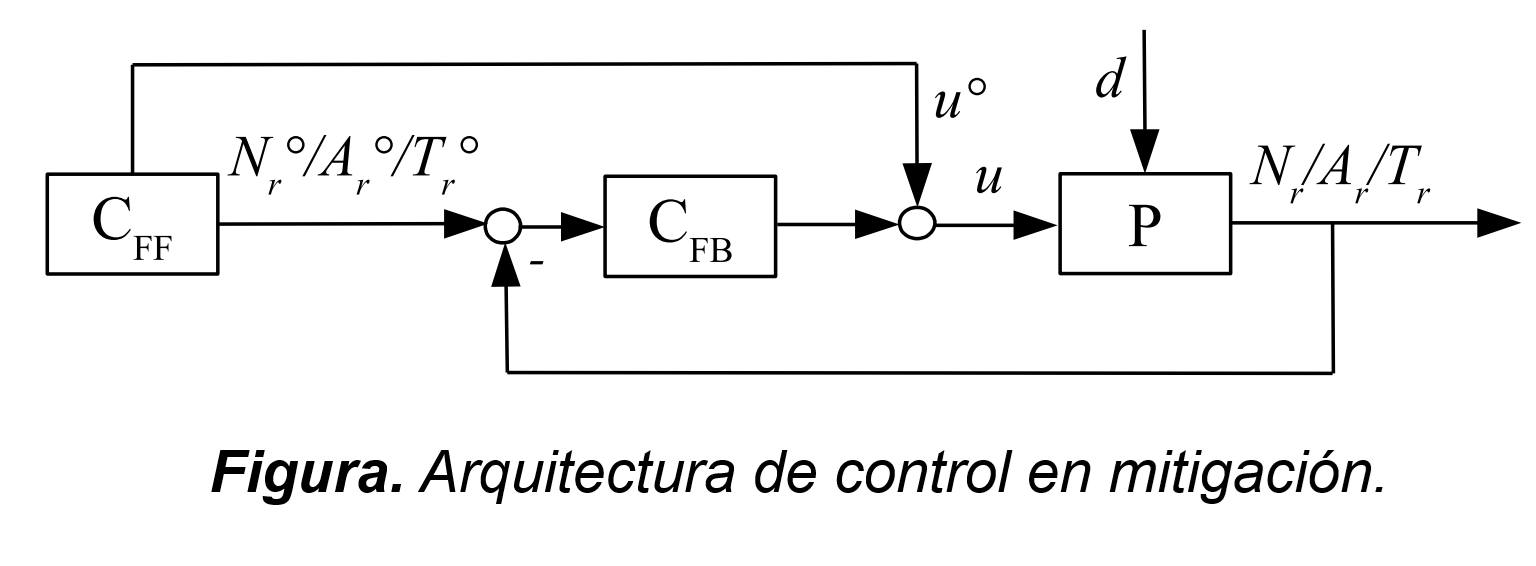
\includegraphics[width=0.70\textwidth]{control-mitigacion.png}
\captionsetup{justification=centering}
\label{C}
\end{figure}

La naturaleza inestable de las trayectorias de estado mientras \( r > 0 \) hace inviable una implementación en lazo abierto de esta política, a menos que se quiera arriesgar a desenfrenos que pueden causar el colapso del sistema de salud pública. 

\vspace{0.3cm}
La trayectoria de referencia debería más bien seguirse adaptando las medidas de políticas públicas \( u(t) \) en tiempo real, basándose en los valores de \( N_r(t) \), \( A_r(t) \), y \( T_r(t) \), que son constantemente monitoreados por las autoridades. Esto corresponde en principio a cerrar un bucle de retroalimentación para estabilizar la trayectoria de referencia inestable.

\end{justify}
\end{frame}


\begin{frame}{Control: Estrategia de Mitigación}
\begin{justify}
\small

\textbf{Diseño del controlador de retroalimentación ideal:}

\vspace{0.2cm}
El modelo final que propone el artículo puede ser linealizado alrededor de la trayectoria de referencia en el tiempo \( t_a \), obteniendo un modelo lineal con coeficientes constantes excepto por los términos \( \beta(u^0(t_a),d(t_a))\) y \( \frac{\partial \beta(u^0(t_a),d(t_a))}{\partial u} \), que dependen de \( t_a \) para trayectorias de referencia de control no triviales \( u^0(t) \). 

\vspace{0.3cm}
Para el análisis subsiguiente, asumimos que estos parámetros cambian en una escala de tiempo mucho más larga que la escala de tiempo de la respuesta de retroalimentación del sistema en lazo cerrado, una suposición común al tratar con control de programación de ganancias, y por lo tanto, los consideramos como constantes con el valor que tienen en el tiempo \( t_a \) alrededor del cual se realiza el análisis de estabilidad de retroalimentación. 
\end{justify}
\end{frame}

\begin{frame}{Control: Estrategia de Mitigación}
\begin{justify}
\small

Las funciones de transferencia del proceso linealizado son entonces:

\vspace{0.3cm}
\[
\frac{\Delta N_r(s)}{\Delta u(t)} = \frac{\mu(t_a)(s + \gamma)}{(s - p(t_a))(s - r(t_a))} e^{-t_m s}
\]
\[
\frac{\Delta A_r(s)}{\Delta u(t)} = \frac{\mu(t_a)(s + (\gamma + \delta))}{(s - p(t_a))(s - r(t_a))(s + \delta)} e^{-t_m s}
\]
\[
\frac{\Delta T_r(s)}{\Delta u(t)} = \frac{\mu(t_a)(s + \gamma)}{(s - p(t_a))(s - r(t_a))} e^{-t_m s}
\]

\vspace{0.3cm}
donde \( \mu(t_a) = \epsilon \frac{\partial \beta(u^0(t_a),d(t_a))}{\partial u} I^0(t_a)\) y \( p(t_a) \) y \( r(t_a) \) son los autovalores del modelo linealizado en \( t = t_a \) alrededor de la trayectoria de referencia.

\end{justify}
\end{frame}

\begin{frame}{Control: Estrategia de Mitigación}
\begin{justify}
\small

Haciendo las suposiciones muy optimistas de que los parámetros \( \epsilon \), \( \gamma \), \( \delta \), y \( t_m \) son constantes y perfectamente conocidos, que la función \( \beta(u, d) \) que expresa los efectos de las decisiones de política pública es perfectamente conocida, decreciente monótona y suave con respecto a \( u \), y que \( d(t) \equiv 0 \), uno puede diseñar el controlador de retroalimentación \( C_{FB} \) como un controlador lineal \( C(s) \) con programación de ganancias, que compensa la no linealidad de la ganancia del proceso, resultando en una dinámica de lazo (aproximadamente) lineal e invariante en el tiempo. 

\vspace{0.3cm}
Al hacerlo, uno también debe tener en cuenta un retraso adicional \( t_c \) de 2 a 4 días dentro del controlador, correspondiente al retraso en la toma de decisiones y la implementación. 
\end{justify}
\end{frame}

\begin{frame}{Control: Estrategia de Mitigación}
\begin{justify}
\small

Asumiendo que uno quiere usar \( N_r(t) \) para control de retroalimentación, la ley de control general es así:

\[
u(t) = u^0(t) + \frac{1}{\mu(t - t_c)} u_f(t - t_c)
\]
\[
u_f(s) = C(s) [N_r^0(s) - N_r(s)]
\]

\vspace{0.3cm}
y la función de transferencia del lazo del sistema controlado es:

\vspace{0.3cm}
\[
L(s) = \frac{C(s) \mu_r(s + \gamma)}{(s - p(t - t_c))(s - r(t - t_c))} e^{-s(t_m + t_c)}
\]

\vspace{0.3cm}
donde \( \mu_r \) es la relación entre el valor actual de la ganancia \( \mu \) de la función de transferencia $\frac{\Delta{N_r (s)}}{\Delta {u(t)}}$ y su valor de referencia usado para la programación de ganancias. En condiciones ideales, \( \mu_r = 1 \), aunque los resultados de los datos experimentales implican que esta ganancia está sujeta a una incertidumbre significativa.
\end{justify}
\end{frame}




\begin{frame}{Experiencia práctica: Simulación del modelo en Python}
\begin{justify}
\small

\begin{figure}[H]
\centering
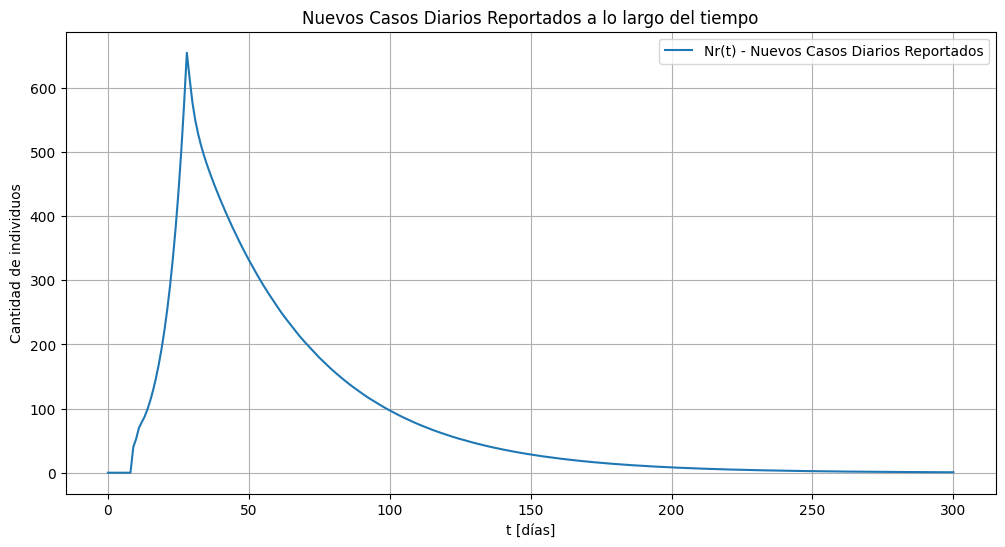
\includegraphics[width=0.90\textwidth]{imagen-2.png}
\captionsetup{justification=centering}
\caption{Comparación del espacio de estado original con el linealizado. Se ocupo el valor de entrada $D_s$ o lo que viene a ser $D=0.35$.}
\label{C2}
\end{figure}

\end{justify}
\end{frame}

\begin{frame}{Definición de la entrada}
\begin{justify}
Se define una entrada: 

$$\beta(u(t), d(t)) = u_{\beta}(t) = \frac{\beta_0}{u(t)}$$ 

\vspace{0.3cm}
Se va a verificar las salidas $N_r$, $A_r$ y $T_r$ para diferentes entradas de $u(t)$. Además, es importante considerar que los rangos de variaciones de la entrada son entre 0 y 1, donde corresponden a un menor y mayor uso de medidas públicas para el control de la pandemia, respectivamente.

\end{justify}
\end{frame}


\begin{frame}{Experiencia práctica: Variación de la Entrada para un $u=0.2$}
\begin{justify}
\small
{\footnotesize
\begin{figure}[H]
\centering
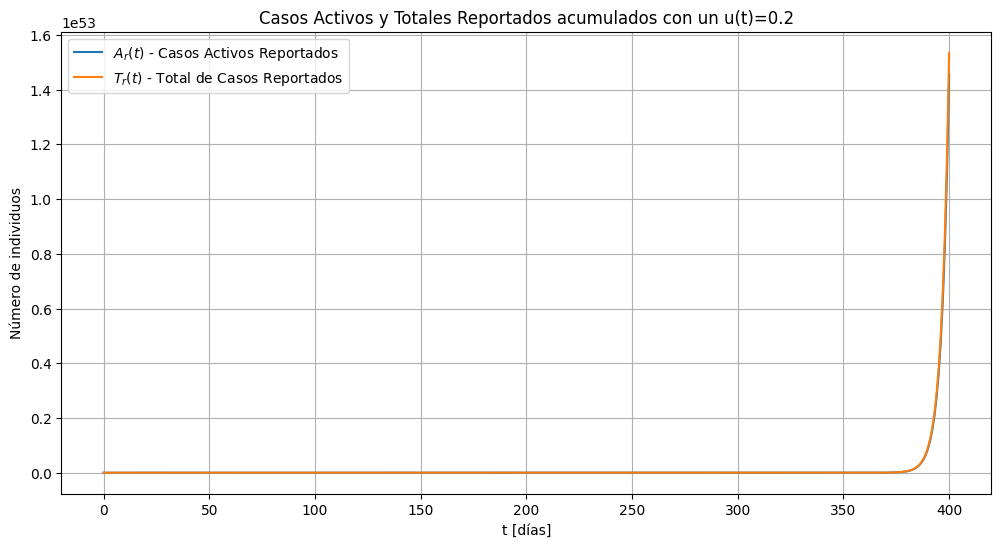
\includegraphics[width=0.5\textwidth]{imagen02-1.png}
\captionsetup{justification=centering}
\label{C2}
\end{figure}

\begin{figure}[H]
\centering
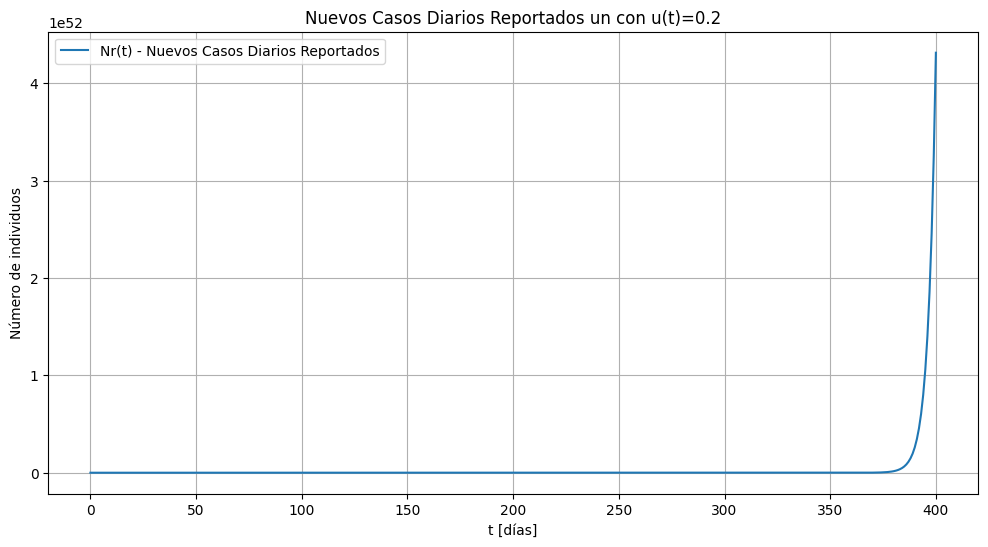
\includegraphics[width=0.5\textwidth]{Imagen02-2.png}
\captionsetup{justification=centering}
\label{C2}
\end{figure}
}
\end{justify}
\end{frame}



\begin{frame}{Experiencia práctica: Variación de la Entrada para un $u=0.5$}
\begin{justify}
\small
{\footnotesize
\begin{figure}[H]
\centering
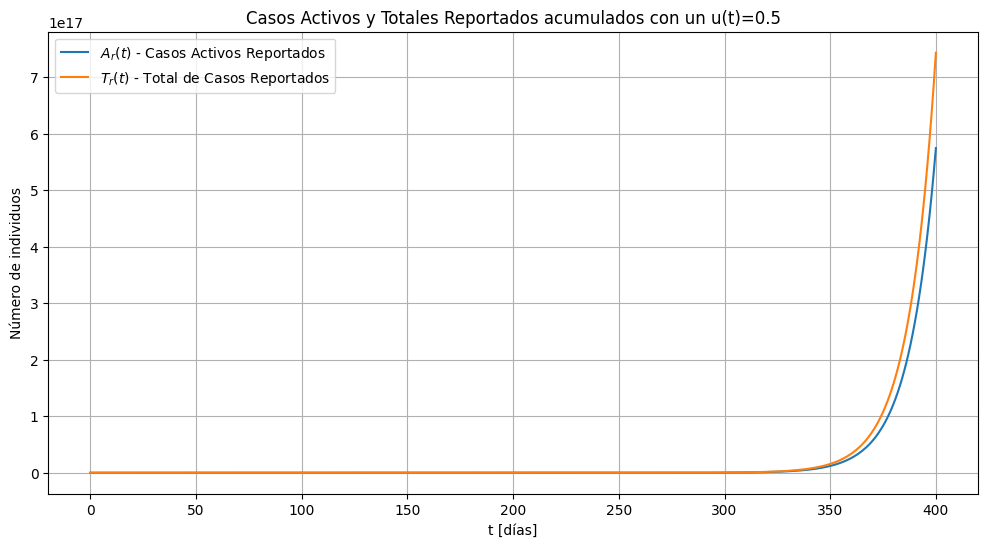
\includegraphics[width=0.5\textwidth]{imagen04-1.png}
\captionsetup{justification=centering}
\label{C2}
\end{figure}

\begin{figure}[H]
\centering
\includegraphics[width=0.5\textwidth]{Imagen05-2.png}
\captionsetup{justification=centering}
\label{C2}
\end{figure}
}
\end{justify}
\end{frame}


\begin{frame}{Experiencia práctica: Variación de la Entrada para un $u=0.7$}
\begin{justify}
\small
{\footnotesize
\begin{figure}[H]
\centering
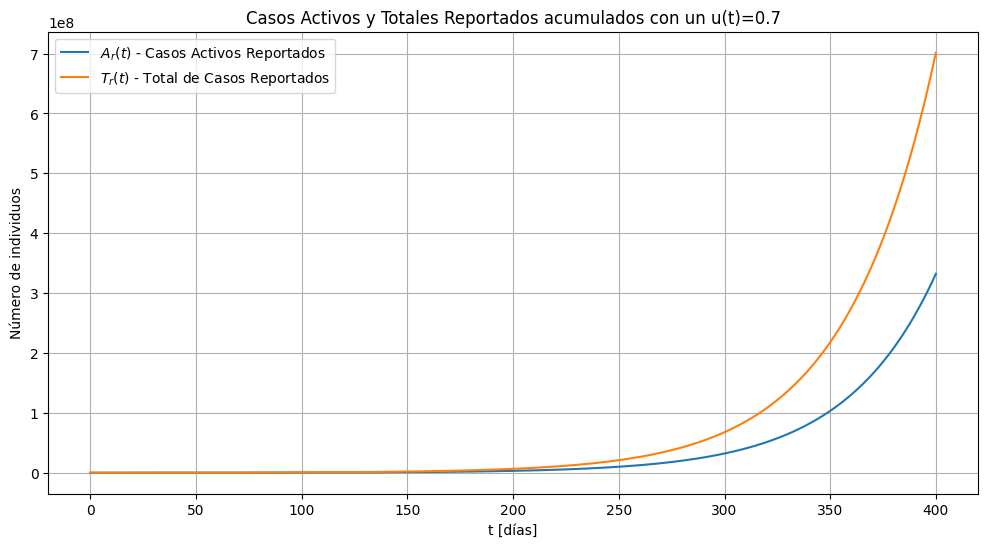
\includegraphics[width=0.5\textwidth]{imagen07-1.png}
\captionsetup{justification=centering}
\label{C2}
\end{figure}

\begin{figure}[H]
\centering
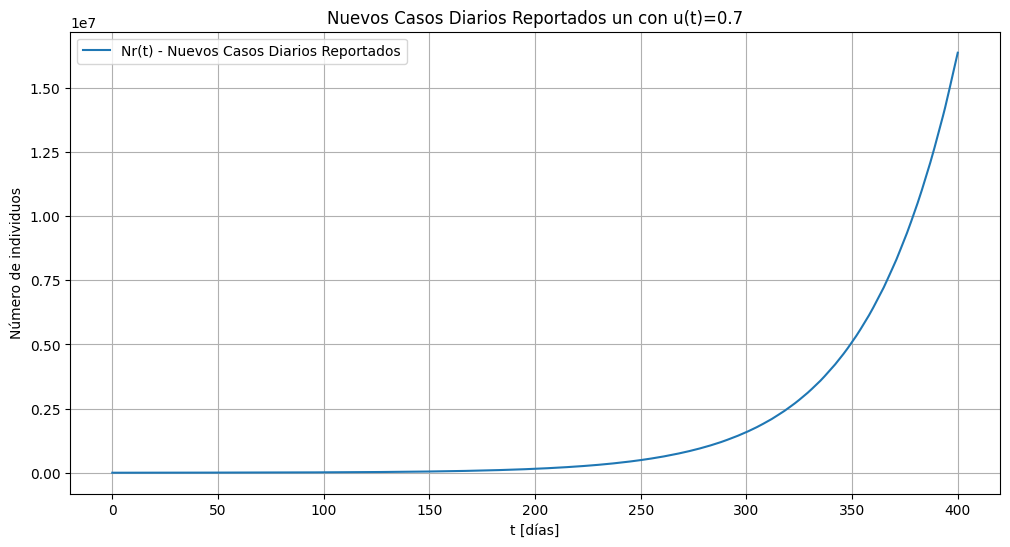
\includegraphics[width=0.5\textwidth]{imagen07-2.png}
\captionsetup{justification=centering}
\label{C2}
\end{figure}
}
\end{justify}
\end{frame}

\begin{frame}{Experiencia practica: Variación de la Entrada para un $u=0.9$}
\begin{justify}
\small
{\footnotesize
\begin{figure}[H]
\centering
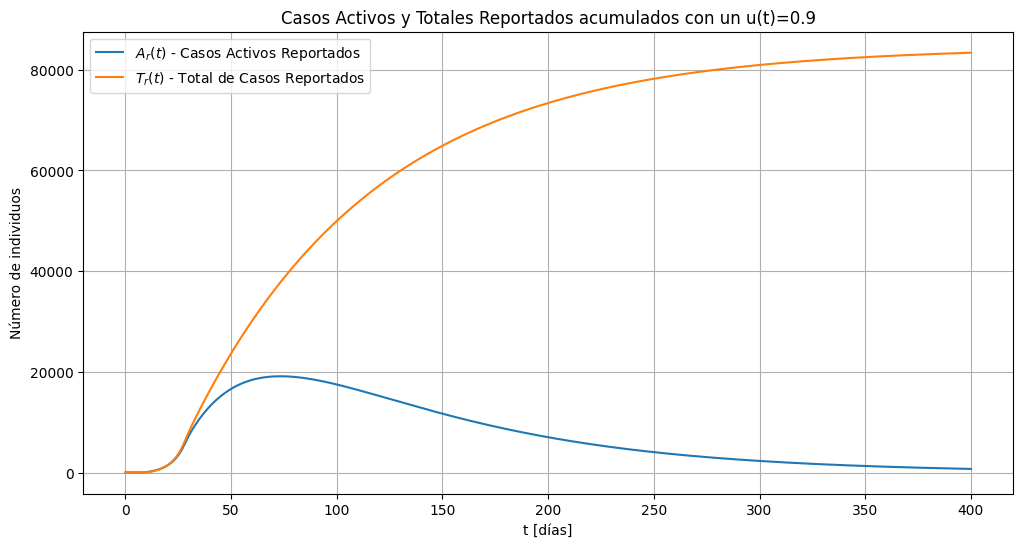
\includegraphics[width=0.5\textwidth]{imagen09-1.png}
\captionsetup{justification=centering}
\label{C2}
\end{figure}

\begin{figure}[H]
\centering
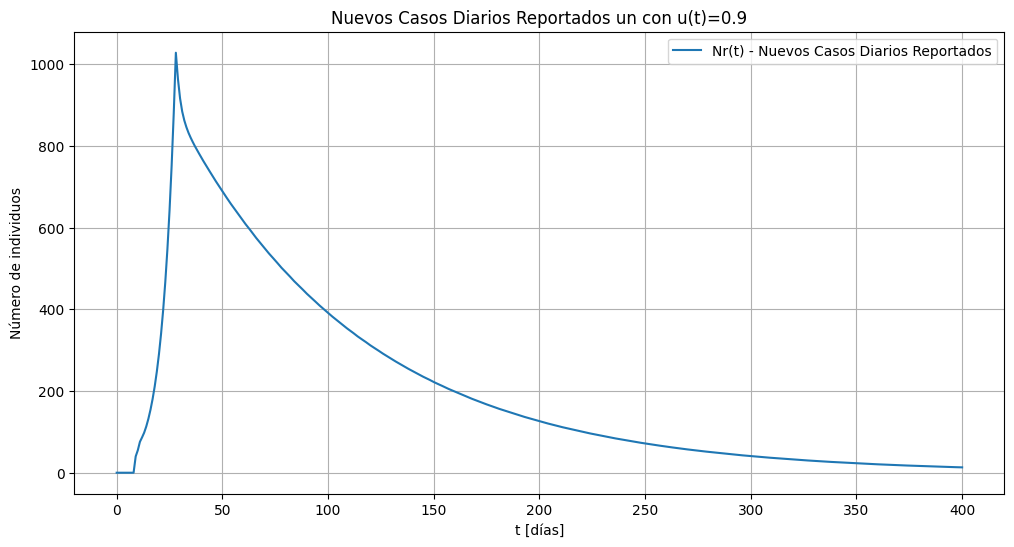
\includegraphics[width=0.5\textwidth]{imagen09-2.png}
\captionsetup{justification=centering}
\label{C2}
\end{figure}
}
\end{justify}
\end{frame}

\section{Linealización y Espacio de estados}
\begin{frame}{Linealización y Espacio de estados}
\begin{justify}
\vspace{0.3cm}
La representación del vector de estado transpuesto se puede observar a continuación:

$$
\mathbf{x}(t)^T = [x_1, x_2, x_3, x_4]
$$

Donde:

\begin{align*}
x_1 = E_t, \quad
x_2 = I_t, \quad
x_3 = L_t, \quad
x_4 = T_t, \quad
u_1 = u_{\beta}(t)
\end{align*}



\end{justify}
\end{frame}



\begin{frame}{Linealización y Espacio de estados}
\begin{justify}
El espacio de estado, se puede obtener linealizando el modelo mediante Taylor de primer orden,
{\footnotesize
$$
\frac{dx_j}{dt} \approx f_i(\mathb {x}_{i}, u_{1}) \approx f_i(\mathbf{x}_{ie}, u_{1e}) + K_{ji}  \Delta x_i + \frac{\partial f_j}{\partial u_1} \Bigg|_{\substack{\mathbf{x_i}=\mathbf{x}_{ie} \\ u_1 =u_{\beta_e}}} \Delta u_{\beta} 
$$

donde

$$ K_{ji} = \frac{\partial f_j}{\partial x_i} \Bigg|_{\substack{\mathbf{x_i}=\mathbf{x}_{ie} \\ u_1 =u_{1e}}}
$$

$$\Delta x_i = x_i - x_{ie}$$
$$\Delta u_{\beta} = u_{\beta} - u_{\beta_e}$$


}
\end{justify}
\end{frame}



\begin{frame}{Linealización y Espacio de estados}
\begin{justify}

{\footnotesize
El modelo de espacio de estado resultante para una salida:

$$Y(t)=[\Delta\dot N_r,  \Delta\dot A_r,  \Delta\dot T_r  ]^T$$

Resultando en,

\begin{align*}
\dot{\mathbf{x}}(t) & = A\mathbf{x}(t) + B\mathbf{u}(t) \\
Y(t) & = C\mathbf{x}(t-\tau_m) \\
\end{align*}

Los vectores $\dot{\mathbf{x}}(t)$, $\mathbf{x}(t)$ y $\mathbf{u}(t)$ resultantes:

$$
\dot{\mathbf{x}}(t)^T = [\Delta  \dot{x}_1, \Delta \dot{x}_2, \Delta \dot{x}_3, \Delta \dot{x}_4]
$$

$$
{\mathbf{x}}(t)^T = [\Delta{x}_1, \Delta {x}_2, \Delta {x}_3, \Delta {x}_4]
$$

$$
{\mathbf{u}}(t) = \Delta u_1
$$
}
\end{justify}
\end{frame}


\begin{frame}{Linealización y Espacio de estados}
\begin{justify}


{\footnotesize

Las matriz estado $A$, la matriz de control $B$ y la matriz de salida $C$, se pueden ver a continuación:

$$
A = \begin{bmatrix}
-\epsilon & u_{\beta_{e}} & 0 & 0  \\
\epsilon & -\gamma & 0 & 0  \\
0 & \gamma  & -\delta & 0 \\
\epsilon & 0 & 0 & 0 \\
\end{bmatrix}
$$

\vspace{0.3cm}

$$
B^T = \begin{bmatrix}
I_{te} & 0 & 0 & 0
\end{bmatrix}
$$

\vspace{0.3cm}

$$
C = \begin{bmatrix}
\epsilon & 0 & 0 & 0  \\
0 & 1 & 1 & 0  \\
0 & 0  & 0 & 1 \\
\end{bmatrix}
$$
}

\end{justify}
\end{frame}



\begin{frame}{Linealización y Espacio de estados}
\begin{justify}


{\footnotesize

Por lo tanto, los puntos de equilibrio se pueden obtener cuando las ecuaciones diferenciales no sufren cambios:


$$\frac{dE_{t}}{dt} = \frac{dI_{t}}{dt} = \frac{dL_{t}}{dt} = \frac{dT_{t}}{dt} = 0$$

por lo tanto,

$$E_{t}=\frac{\beta_{0}}{\epsilon u_e}I_{t}$$

$$I_{t}=\frac{\epsilon}{\gamma}E_{t}$$

$$L_{t}=\frac{\gamma}{\delta}I_{t}$$

$$T_{t} = 0 $$

Para encontrar un punto de equilibrio solo basta encontrar $I_{t}$.
}

\end{justify}
\end{frame}


%\begin{frame}{Derivación del modelo}
%\begin{justify}
%\small
% El modelo orientado al control puede formularse como un sistema en espacio de estados con salidas de retardo
%{\footnotesize
%\begin{align}
 %   \frac{dE_t}{dt} &= \beta(u(t), d(t))I_t - \epsilon E_t, \label{eq:Et} \\[10pt]
%   \frac{dI_t}{dt} &= \epsilon E_t - \gamma I_t, \label{eq:It} \\[10pt]
%    \frac{dL_t}{dt} &= \gamma I_t - \delta L_t, \label{eq:Lt} \\[10pt]
%   \frac{dT_t}{dt} &= \epsilon E_t, \label{eq:Tt} \\[10pt]
 %   N_r(t) &= \epsilon E_t(t - \tau_m), \label{eq:Nrt} \\[10pt]
%    A_r(t) &= I_t(t - \tau_m) + L_t(t - \tau_m), \label{eq:Art} \\[10pt]
%    T_r(t) &= T_t(t - \tau_m). \label{eq:Trt}
%\end{align}
%}
%\end{justify}
%\end{frame}

\section{Teoría: Control Predictivo GPC}
\begin{frame}{Control Predictivo GPC}
\begin{justify}
\vspace{0.3cm}
\begin{itemize}
  Hay tres componentes principales en el diseño de un GPC:
    \item Un modelo del sistema a controlar: Este modelo se utiliza para predecir la salida del sistema durante el horizonte de predicción.
    \item Formulación de la función criterio.
    \item Minimización de la función de criterio para producir la secuencia de salida de control óptima durante el horizonte de predicción.
\end{itemize}
\end{justify}
\end{frame}

\begin{frame}{Control Predictivo GPC}
\begin{justify}
\vspace{0.3cm}
\begin{itemize}
   \item Considera una ecuación descrita por el sistema de estado lineal:
   $x(t+1)=Ax(t)+Bu(t)$\\
   $y(t)=Hx(t)$
\item Donde $x(t) \in R^n, y(t) \in R^r y u(t) \in R^m$ son el estado.
\item A, B y H son matrices con dimensiones apropiadas.
\item La estructura de este modelo es usado para formular controles predictivos. Primero se define un modelo de predicción de estado de la forma:
\\
$\hat{x}(t+j/t)=A\hat{x}(t+j-1/t)+Bu(t+j-1/t), j=1. 2. ....., p, $ 
\\
Donde $\hat{x}(t+j/t)$ denota el vector de predicción en el instante t para  el instante t+j h(./t) denota la secuencia del control de vectores en el intervalo de prediccion. 
\end{itemize}
\end{justify}
\end{frame}

\begin{frame}{Control Predictivo GPC}
\begin{justify}
\vspace{0.3cm}
\begin{itemize}
Este modelo es redefinido para cada instante de muestra t  del actual estado de vector y el control previamente aplicado.
$\hat{x}(t/t)=x(t); u(t-j/t)=u(t-j); j=1,2,...,h.$
\\
Aplicando la ecuacion anterior recursivamente a las condiciones iniciales, las siguientes ecuaciones pueden ser obtenidos:
$\hat{y}(t+1/t)= HAx(t)+HBu(t)$
$\hat{y}(t+2/t)= HA^2x(t)+HABu(t)+HBu(t+1),$
.
.
.
$\hat{y}(t+p_1/t)=HA^{p1}x(t)+HP^{p1-1}Bu(t)+...+HP^{p1-p2-1}Bu(t+p_2)$

\end{itemize}
\end{justify}
\end{frame}

\begin{frame}{Control Predictivo GPC}
\begin{justify}
\vspace{0.3cm}
\begin{itemize}
Una forma reducida de escribir esta ecuacion es de la siguiente manera:
$Y=Gx(t)+F_1 U$
\\ 
Donde:
\centering
\hfill \break
$Y=\begin{bmatrix}\hat{y}(t+1/t) &\hat{y}(t+2/t)&...& \hat{y}(t+p_1/t)]^T
\end{bmatrix}$ 
\\
\hfill \break
\\
$G=
\begin{bmatrix}
    HA \\
    HA^2\\
    . \\
    .\\
    HA^{p_1}
\end{bmatrix}$
\end{itemize}
\end{justify}
\end{frame}

\begin{frame}{Control Predictivo GPC}
\begin{justify}
\vspace{0.3cm}
\begin{itemize}
\centering
$F_1=
\begin{bmatrix}
    HB & 0 & ... & 0 \\
    HAB & HB & ... & 0\\
    . & . & ... & . \\
    . & . & ... & . \\
    . & . & ... & . \\
    HA^{p_1-1} & HA^{p_1-2}B & ... & HA^{p_1-p_2-1}B
\end{bmatrix}
$
\\
\hfill \break
\\
$U=\begin{bmatrix}u(t)& u(t+1)&...& u(t+p_2)\end{bmatrix}^T$ 
\\

\end{itemize}
\end{justify}
\end{frame}

\begin{frame}{Minimización función de costo}
\begin{justify}
\vspace{0.3cm}
\begin{itemize}
\item La ley de control predictivo generalmente se formula para minimizar una función de costos, también llamada criterio de desempeño.
\item Un criterio de desempeño simple que se puede utilizar en el diseño de control predictivo está dado por:
\\
\centering
\item $J=\frac{1}{2}\sum_{j=1}^{p1}\left [ y_d (t+j)-\hat{y}(t+j)\right ]^TQ_j\left [ y_d(t+j)-\hat{y}(t+j)] \right ]$
\\
o
\\
\item $J=\frac{1}{2}(Y_d-Y)^T Q(Y_d-Y)$
\\
\hfill \break
\justifying
Donde $Y_d(t + j), j = 1,2, ...,P_l$, es una trayectoria de referencia para el vector de salida que puede redefinirse en cada instante de muestreo t, y Q es una matriz definida no negativa.
\end{itemize}
\end{justify}
\end{frame}

\begin{frame}{Minimización función de costo}
\begin{justify}
\vspace{0.3cm}
\begin{itemize}
\item La solución que minimiza el índice de desempeño se puede obtener resolviendo:
\\
\centering
$\frac{\partial J}{\partial U}=0$
\item Del cual se pueden obtener cálculos directos explícitamente como:
\\
\hfill \break
$U=(F_1^TQF_1)^{-1}F_1^{T}Q[Y_d-Gx(t)]$
\\
\hfill \break
\justifying
Bajo la condición de que la secuencia de control permanezca constante durante el intervalo de predicción, es decir,
$u(t)=u(t+1)=...=u(t+p_1),$
\end{itemize}
\end{justify}
\end{frame}

\begin{frame}{Minimización función de costo}
\begin{justify}
\vspace{0.3cm}
\begin{itemize}
\item La accion de control obtenida es:
\\
$U=(\bar{F_1}^TQ\bar{F_1})^{-1}\bar{F_1}^{T}Q[Y_d-Gx(t)]$
\\
\hfill \break
Donde:
\\
\centering
$\bar{F}=
\begin{bmatrix}
    HB \\
    HAB+HB\\
    . \\
    .\\
    .\\
    H(A^{p_1-1}+A^{p1-2}+...+I)B
\end{bmatrix}$
\\
\justifying
\item En este caso, el horizonte de predicción $p_1$ afecta a $u(t)$ en la ley de control.
\end{itemize}
\end{justify}
\end{frame}


\begin{frame}{Minimización función de costo}
\begin{justify}
\vspace{0.3cm}
\begin{itemize}
\item Otra forma común de resolver el problema del control predictivo es utilizar incrementos de control en lugar de la salida de control en:
\\
\hfill \break
\item $J=\frac{1}{2}\sum_{j=1}^{p1}\left [ y_d (t+j)-\hat{y}(t+j)\right ]^TQ_j\left [ y_d(t+j)-\hat{y}(t+j) \right ]+ \frac{1}{2}\sum_{j=1}^{p_2}\Delta u(t+j)^T R_j \Delta u (t+j)$ o
\hfill \break
\item $J=\frac{1}{2}(Y_d-Y)^T Q(Y_d-Y)+\Delta U^TR\Delta U$
\\
\hfill \break
Donde $Y_d(t + j), j = 1,2, ...,p_l$, es una trayectoria de referencia para el vector de salida que puede redefinirse en cada instante de muestreo t, y Q es una matriz definida no negativa.
\end{itemize}
\end{justify}
\end{frame}

\begin{frame}{Minimización función de costo}
\begin{justify}
\vspace{0.3cm}
\begin{itemize}
Este criterio de rendimiento se utiliza en muchos controladores predictivos. Para hacer frente a los incrementos de control en lugar de la salida de control, la ecuación compuesta se puede reescribir como:
\\
\item $Y=Gx(t)+F_{11}\Delta U + F_2 u(t-1)$
\\
Donde:
\\
\centering
$F_{11}=
\begin{bmatrix}
    HB & 0 & ... & 0 \\
    H(A+I)B & HB & ... & 0\\
    . & . & ... & . \\
    . & . & ... & . \\
    . & . & ... & . \\
    H\lambda(p_2)B & H\lambda(p_2-1)B & ... HA^{p_1-p_2-1}B
\end{bmatrix}$
\\
$\Delta U =
\begin{bmatrix}
    \Delta u(t) & \Delta u(t+1) & ... & \Delta u(t+p_2)
\end{bmatrix}^T$
\end{itemize}
\end{justify}
\end{frame}


\begin{frame}{Minimización función de costo}
\begin{justify}
\vspace{0.3cm}
\begin{itemize}
\\
\centering
$F_{2}=
\begin{bmatrix}
    HB \\
    H(A+I)B\\
    . \\
    . \\
    . \\
    H(A^(p_1-1)+ A^(p_1-2)+... +A^{p_1-p_2-1})B
\end{bmatrix}$
\\
\hfill \break
$\lambda (j) =\sum_{k=o}^{k=j} A^{p_1-p_2-1+k}$
\\
\hfill \break
Sustituyendo quedaría:
\hfill \break
\centering
$ \Delta U = (F_{11}^T Q F_{11}+\lambda I)^{-1}F_{11}^T Q  \left [ Y_d-Gx(t)-F_2 u (t-1)  \right ] $
\end{itemize}
\end{justify}
\end{frame}


\begin{frame}{Minimización función de costo}
\begin{justify}
\vspace{0.3cm}
\begin{itemize}
Aunque la ecuación anterior proporciona la secuencia de control completa minimizando J sobre el horizonte de predicción, sólo los valores de las primeras m filas en realidad se aplican al sistema como señal de control. Por tanto, la ley de control final tiene la forma:
\\
\hfill \break
 $\Delta u(t)=g_1 \left [ Y_d- Gx(t)-F_2 u(t-1) \right ]$,
 \\
 con:
 \\
 $g_1=\left [T_m, 0, 0, ..., 0  \right ](F_{11}^T Q F_{11}+R)^{-1} F_{11}^T Q)$ 
\hfill \break

 Siendo las primeras m filas de la matriz:
 \\
 \centering
 $(F_{11}^T Q F_{11}+R)^{-1} F_{11}^T Q)$
\end{itemize}
\end{justify}
\end{frame}


\begin{frame}{Minimización función de costo}
\begin{justify}
\vspace{0.3cm}
\begin{itemize}
En general, el criterio de desempeño impone un compromiso entre que la salida del sistema esté lo más cerca posible de la trayectoria de referencia y que la acción de control requerida no sea excesiva. Usando un criterio más simple, la dimensión del problema de control puede reducirse a expensas de alguna pérdida en el desempeño.
\end{itemize}
\end{justify}
\end{frame}

\end{document}